% Graphic for TeX using PGF
% Title: /home/satenske/cours/AP/obj3/uml16.dia
% Creator: Dia v0.97.1
% CreationDate: Thu Sep 22 10:19:53 2011
% For: satenske
% \usepackage{tikz}
% The following commands are not supported in PSTricks at present
% We define them conditionally, so when they are implemented,
% this pgf file will use them.
\ifx\du\undefined
  \newlength{\du}
\fi
\setlength{\du}{15\unitlength}
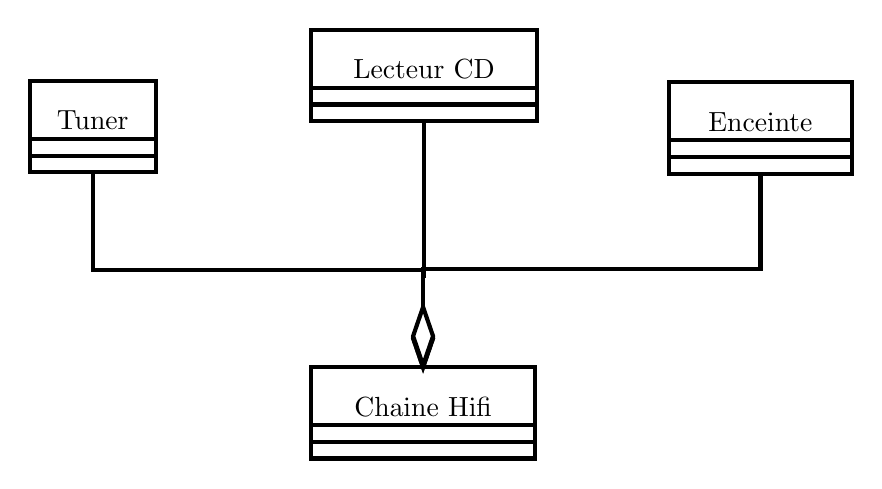
\begin{tikzpicture}
\pgftransformxscale{1.000000}
\pgftransformyscale{-1.000000}
\definecolor{dialinecolor}{rgb}{0.000000, 0.000000, 0.000000}
\pgfsetstrokecolor{dialinecolor}
\definecolor{dialinecolor}{rgb}{1.000000, 1.000000, 1.000000}
\pgfsetfillcolor{dialinecolor}
\pgfsetlinewidth{0.100000\du}
\pgfsetdash{}{0pt}
\definecolor{dialinecolor}{rgb}{1.000000, 1.000000, 1.000000}
\pgfsetfillcolor{dialinecolor}
\fill (8.200000\du,5.650000\du)--(8.200000\du,7.050000\du)--(11.235000\du,7.050000\du)--(11.235000\du,5.650000\du)--cycle;
\definecolor{dialinecolor}{rgb}{0.000000, 0.000000, 0.000000}
\pgfsetstrokecolor{dialinecolor}
\draw (8.200000\du,5.650000\du)--(8.200000\du,7.050000\du)--(11.235000\du,7.050000\du)--(11.235000\du,5.650000\du)--cycle;
% setfont left to latex
\definecolor{dialinecolor}{rgb}{0.000000, 0.000000, 0.000000}
\pgfsetstrokecolor{dialinecolor}
\node at (9.717500\du,6.600000\du){Tuner};
\definecolor{dialinecolor}{rgb}{1.000000, 1.000000, 1.000000}
\pgfsetfillcolor{dialinecolor}
\fill (8.200000\du,7.050000\du)--(8.200000\du,7.450000\du)--(11.235000\du,7.450000\du)--(11.235000\du,7.050000\du)--cycle;
\definecolor{dialinecolor}{rgb}{0.000000, 0.000000, 0.000000}
\pgfsetstrokecolor{dialinecolor}
\draw (8.200000\du,7.050000\du)--(8.200000\du,7.450000\du)--(11.235000\du,7.450000\du)--(11.235000\du,7.050000\du)--cycle;
\definecolor{dialinecolor}{rgb}{1.000000, 1.000000, 1.000000}
\pgfsetfillcolor{dialinecolor}
\fill (8.200000\du,7.450000\du)--(8.200000\du,7.850000\du)--(11.235000\du,7.850000\du)--(11.235000\du,7.450000\du)--cycle;
\definecolor{dialinecolor}{rgb}{0.000000, 0.000000, 0.000000}
\pgfsetstrokecolor{dialinecolor}
\draw (8.200000\du,7.450000\du)--(8.200000\du,7.850000\du)--(11.235000\du,7.850000\du)--(11.235000\du,7.450000\du)--cycle;
\pgfsetlinewidth{0.100000\du}
\pgfsetdash{}{0pt}
\definecolor{dialinecolor}{rgb}{1.000000, 1.000000, 1.000000}
\pgfsetfillcolor{dialinecolor}
\fill (14.975000\du,4.415000\du)--(14.975000\du,5.815000\du)--(20.422500\du,5.815000\du)--(20.422500\du,4.415000\du)--cycle;
\definecolor{dialinecolor}{rgb}{0.000000, 0.000000, 0.000000}
\pgfsetstrokecolor{dialinecolor}
\draw (14.975000\du,4.415000\du)--(14.975000\du,5.815000\du)--(20.422500\du,5.815000\du)--(20.422500\du,4.415000\du)--cycle;
% setfont left to latex
\definecolor{dialinecolor}{rgb}{0.000000, 0.000000, 0.000000}
\pgfsetstrokecolor{dialinecolor}
\node at (17.698750\du,5.365000\du){Lecteur CD};
\definecolor{dialinecolor}{rgb}{1.000000, 1.000000, 1.000000}
\pgfsetfillcolor{dialinecolor}
\fill (14.975000\du,5.815000\du)--(14.975000\du,6.215000\du)--(20.422500\du,6.215000\du)--(20.422500\du,5.815000\du)--cycle;
\definecolor{dialinecolor}{rgb}{0.000000, 0.000000, 0.000000}
\pgfsetstrokecolor{dialinecolor}
\draw (14.975000\du,5.815000\du)--(14.975000\du,6.215000\du)--(20.422500\du,6.215000\du)--(20.422500\du,5.815000\du)--cycle;
\definecolor{dialinecolor}{rgb}{1.000000, 1.000000, 1.000000}
\pgfsetfillcolor{dialinecolor}
\fill (14.975000\du,6.215000\du)--(14.975000\du,6.615000\du)--(20.422500\du,6.615000\du)--(20.422500\du,6.215000\du)--cycle;
\definecolor{dialinecolor}{rgb}{0.000000, 0.000000, 0.000000}
\pgfsetstrokecolor{dialinecolor}
\draw (14.975000\du,6.215000\du)--(14.975000\du,6.615000\du)--(20.422500\du,6.615000\du)--(20.422500\du,6.215000\du)--cycle;
\pgfsetlinewidth{0.100000\du}
\pgfsetdash{}{0pt}
\definecolor{dialinecolor}{rgb}{1.000000, 1.000000, 1.000000}
\pgfsetfillcolor{dialinecolor}
\fill (23.600000\du,5.680000\du)--(23.600000\du,7.080000\du)--(28.005000\du,7.080000\du)--(28.005000\du,5.680000\du)--cycle;
\definecolor{dialinecolor}{rgb}{0.000000, 0.000000, 0.000000}
\pgfsetstrokecolor{dialinecolor}
\draw (23.600000\du,5.680000\du)--(23.600000\du,7.080000\du)--(28.005000\du,7.080000\du)--(28.005000\du,5.680000\du)--cycle;
% setfont left to latex
\definecolor{dialinecolor}{rgb}{0.000000, 0.000000, 0.000000}
\pgfsetstrokecolor{dialinecolor}
\node at (25.802500\du,6.630000\du){Enceinte};
\definecolor{dialinecolor}{rgb}{1.000000, 1.000000, 1.000000}
\pgfsetfillcolor{dialinecolor}
\fill (23.600000\du,7.080000\du)--(23.600000\du,7.480000\du)--(28.005000\du,7.480000\du)--(28.005000\du,7.080000\du)--cycle;
\definecolor{dialinecolor}{rgb}{0.000000, 0.000000, 0.000000}
\pgfsetstrokecolor{dialinecolor}
\draw (23.600000\du,7.080000\du)--(23.600000\du,7.480000\du)--(28.005000\du,7.480000\du)--(28.005000\du,7.080000\du)--cycle;
\definecolor{dialinecolor}{rgb}{1.000000, 1.000000, 1.000000}
\pgfsetfillcolor{dialinecolor}
\fill (23.600000\du,7.480000\du)--(23.600000\du,7.880000\du)--(28.005000\du,7.880000\du)--(28.005000\du,7.480000\du)--cycle;
\definecolor{dialinecolor}{rgb}{0.000000, 0.000000, 0.000000}
\pgfsetstrokecolor{dialinecolor}
\draw (23.600000\du,7.480000\du)--(23.600000\du,7.880000\du)--(28.005000\du,7.880000\du)--(28.005000\du,7.480000\du)--cycle;
\pgfsetlinewidth{0.100000\du}
\pgfsetdash{}{0pt}
\definecolor{dialinecolor}{rgb}{1.000000, 1.000000, 1.000000}
\pgfsetfillcolor{dialinecolor}
\fill (14.975000\du,12.545000\du)--(14.975000\du,13.945000\du)--(20.375000\du,13.945000\du)--(20.375000\du,12.545000\du)--cycle;
\definecolor{dialinecolor}{rgb}{0.000000, 0.000000, 0.000000}
\pgfsetstrokecolor{dialinecolor}
\draw (14.975000\du,12.545000\du)--(14.975000\du,13.945000\du)--(20.375000\du,13.945000\du)--(20.375000\du,12.545000\du)--cycle;
% setfont left to latex
\definecolor{dialinecolor}{rgb}{0.000000, 0.000000, 0.000000}
\pgfsetstrokecolor{dialinecolor}
\node at (17.675000\du,13.495000\du){Chaine Hifi};
\definecolor{dialinecolor}{rgb}{1.000000, 1.000000, 1.000000}
\pgfsetfillcolor{dialinecolor}
\fill (14.975000\du,13.945000\du)--(14.975000\du,14.345000\du)--(20.375000\du,14.345000\du)--(20.375000\du,13.945000\du)--cycle;
\definecolor{dialinecolor}{rgb}{0.000000, 0.000000, 0.000000}
\pgfsetstrokecolor{dialinecolor}
\draw (14.975000\du,13.945000\du)--(14.975000\du,14.345000\du)--(20.375000\du,14.345000\du)--(20.375000\du,13.945000\du)--cycle;
\definecolor{dialinecolor}{rgb}{1.000000, 1.000000, 1.000000}
\pgfsetfillcolor{dialinecolor}
\fill (14.975000\du,14.345000\du)--(14.975000\du,14.745000\du)--(20.375000\du,14.745000\du)--(20.375000\du,14.345000\du)--cycle;
\definecolor{dialinecolor}{rgb}{0.000000, 0.000000, 0.000000}
\pgfsetstrokecolor{dialinecolor}
\draw (14.975000\du,14.345000\du)--(14.975000\du,14.745000\du)--(20.375000\du,14.745000\du)--(20.375000\du,14.345000\du)--cycle;
\pgfsetlinewidth{0.100000\du}
\pgfsetdash{}{0pt}
\pgfsetmiterjoin
\pgfsetbuttcap
{
\definecolor{dialinecolor}{rgb}{0.000000, 0.000000, 0.000000}
\pgfsetfillcolor{dialinecolor}
% was here!!!
\definecolor{dialinecolor}{rgb}{0.000000, 0.000000, 0.000000}
\pgfsetstrokecolor{dialinecolor}
\draw (17.675000\du,12.545000\du)--(17.675000\du,10.197500\du)--(9.717500\du,10.197500\du)--(9.717500\du,7.850000\du);
}
\definecolor{dialinecolor}{rgb}{0.000000, 0.000000, 0.000000}
\pgfsetstrokecolor{dialinecolor}
\draw (17.675000\du,11.286421\du)--(17.675000\du,10.197500\du)--(9.717500\du,10.197500\du)--(9.717500\du,7.850000\du);
\pgfsetdash{}{0pt}
\pgfsetmiterjoin
\pgfsetbuttcap
\definecolor{dialinecolor}{rgb}{1.000000, 1.000000, 1.000000}
\pgfsetfillcolor{dialinecolor}
\fill (17.675000\du,12.545000\du)--(17.435000\du,11.845000\du)--(17.675000\du,11.145000\du)--(17.915000\du,11.845000\du)--cycle;
\pgfsetlinewidth{0.100000\du}
\pgfsetdash{}{0pt}
\pgfsetmiterjoin
\pgfsetbuttcap
\definecolor{dialinecolor}{rgb}{0.000000, 0.000000, 0.000000}
\pgfsetstrokecolor{dialinecolor}
\draw (17.675000\du,12.545000\du)--(17.435000\du,11.845000\du)--(17.675000\du,11.145000\du)--(17.915000\du,11.845000\du)--cycle;
% setfont left to latex
\definecolor{dialinecolor}{rgb}{0.000000, 0.000000, 0.000000}
\pgfsetstrokecolor{dialinecolor}
\node at (13.696250\du,9.997500\du){};
\definecolor{dialinecolor}{rgb}{0.000000, 0.000000, 0.000000}
\pgfsetstrokecolor{dialinecolor}
\node[anchor=west] at (18.225000\du,12.345000\du){};
\definecolor{dialinecolor}{rgb}{0.000000, 0.000000, 0.000000}
\pgfsetstrokecolor{dialinecolor}
\node[anchor=west] at (9.917500\du,8.450000\du){};
\pgfsetlinewidth{0.100000\du}
\pgfsetdash{}{0pt}
\pgfsetmiterjoin
\pgfsetbuttcap
{
\definecolor{dialinecolor}{rgb}{0.000000, 0.000000, 0.000000}
\pgfsetfillcolor{dialinecolor}
% was here!!!
\definecolor{dialinecolor}{rgb}{0.000000, 0.000000, 0.000000}
\pgfsetstrokecolor{dialinecolor}
\draw (17.675000\du,12.545000\du)--(17.675000\du,10.350000\du)--(17.698800\du,10.350000\du)--(17.698800\du,6.615000\du);
}
\definecolor{dialinecolor}{rgb}{0.000000, 0.000000, 0.000000}
\pgfsetstrokecolor{dialinecolor}
\draw (17.675000\du,11.286421\du)--(17.675000\du,10.350000\du)--(17.698800\du,10.350000\du)--(17.698800\du,6.615000\du);
\pgfsetdash{}{0pt}
\pgfsetmiterjoin
\pgfsetbuttcap
\definecolor{dialinecolor}{rgb}{1.000000, 1.000000, 1.000000}
\pgfsetfillcolor{dialinecolor}
\fill (17.675000\du,12.545000\du)--(17.435000\du,11.845000\du)--(17.675000\du,11.145000\du)--(17.915000\du,11.845000\du)--cycle;
\pgfsetlinewidth{0.100000\du}
\pgfsetdash{}{0pt}
\pgfsetmiterjoin
\pgfsetbuttcap
\definecolor{dialinecolor}{rgb}{0.000000, 0.000000, 0.000000}
\pgfsetstrokecolor{dialinecolor}
\draw (17.675000\du,12.545000\du)--(17.435000\du,11.845000\du)--(17.675000\du,11.145000\du)--(17.915000\du,11.845000\du)--cycle;
% setfont left to latex
\definecolor{dialinecolor}{rgb}{0.000000, 0.000000, 0.000000}
\pgfsetstrokecolor{dialinecolor}
\node at (17.686900\du,10.150000\du){};
\definecolor{dialinecolor}{rgb}{0.000000, 0.000000, 0.000000}
\pgfsetstrokecolor{dialinecolor}
\node[anchor=west] at (18.225000\du,12.345000\du){};
\definecolor{dialinecolor}{rgb}{0.000000, 0.000000, 0.000000}
\pgfsetstrokecolor{dialinecolor}
\node[anchor=west] at (17.898800\du,7.215000\du){};
\pgfsetlinewidth{0.100000\du}
\pgfsetdash{}{0pt}
\pgfsetmiterjoin
\pgfsetbuttcap
{
\definecolor{dialinecolor}{rgb}{0.000000, 0.000000, 0.000000}
\pgfsetfillcolor{dialinecolor}
% was here!!!
\definecolor{dialinecolor}{rgb}{0.000000, 0.000000, 0.000000}
\pgfsetstrokecolor{dialinecolor}
\draw (17.675000\du,12.494719\du)--(17.675000\du,10.187360\du)--(25.802500\du,10.187360\du)--(25.802500\du,7.880000\du);
}
\definecolor{dialinecolor}{rgb}{0.000000, 0.000000, 0.000000}
\pgfsetstrokecolor{dialinecolor}
\draw (17.675000\du,11.236141\du)--(17.675000\du,10.187360\du)--(25.802500\du,10.187360\du)--(25.802500\du,7.880000\du);
\pgfsetdash{}{0pt}
\pgfsetmiterjoin
\pgfsetbuttcap
\definecolor{dialinecolor}{rgb}{1.000000, 1.000000, 1.000000}
\pgfsetfillcolor{dialinecolor}
\fill (17.675000\du,12.494719\du)--(17.435000\du,11.794719\du)--(17.675000\du,11.094719\du)--(17.915000\du,11.794719\du)--cycle;
\pgfsetlinewidth{0.100000\du}
\pgfsetdash{}{0pt}
\pgfsetmiterjoin
\pgfsetbuttcap
\definecolor{dialinecolor}{rgb}{0.000000, 0.000000, 0.000000}
\pgfsetstrokecolor{dialinecolor}
\draw (17.675000\du,12.494719\du)--(17.435000\du,11.794719\du)--(17.675000\du,11.094719\du)--(17.915000\du,11.794719\du)--cycle;
% setfont left to latex
\definecolor{dialinecolor}{rgb}{0.000000, 0.000000, 0.000000}
\pgfsetstrokecolor{dialinecolor}
\node at (21.738750\du,9.987360\du){};
\definecolor{dialinecolor}{rgb}{0.000000, 0.000000, 0.000000}
\pgfsetstrokecolor{dialinecolor}
\node[anchor=west] at (18.225000\du,12.294719\du){};
\definecolor{dialinecolor}{rgb}{0.000000, 0.000000, 0.000000}
\pgfsetstrokecolor{dialinecolor}
\node[anchor=west] at (26.002500\du,8.480000\du){};
\end{tikzpicture}
